\documentclass[11pt]{article}

\usepackage{booktabs}
\usepackage{homeworkpkg}
\usepackage{enumitem}
\usepackage{xcolor,listings}
\usepackage{caption}
\usepackage{multirow}
\usepackage{multicol}

\graphicspath{ {images/} }

%% Local Macros and packages: add any of your own definitions here.

\begin{document}

% Homework number, your name and NetID, and optionally, the names/NetIDs of anyone you collaborated with. If you did not collaborate with anybody, leave the last parameter empty.
\homework
    {3}
    {Nestor Alejandro Bermudez Sarmiento (nab6)}
    {}

Assignment 3 focuses on the Naive Bayes classification method. This report shows the performance of such method against different datasets and different feature extraction methods. I'm using Python 3.6 for my implementation.

\section*{Part 1}

In this section we will take ASCII representations of digits to train our model and then evaluate its performance with a different of examples in the same format.

\subsubsection*{Implementation details}
My code is split in the following pieces:\\

\textbf{Parser}: this class takes care of interfacing with the text file. It takes the paths for the files that contain the data and labels and generates tuples formed with a matrix representation of an example and its corresponding label. The class itself is a Python generator to prevent blowing up the memory (not that it will happen with the given dataset).\\

\textbf{Feature Extractors}: I created multiple of these classes that I call 'Feature extractors', they basically take an item and generate an array of features that will then be fed into the classifier. For Part 1.1 I created the \textbf{SinglePixelFeatureExtractor} which simply maps every pixel into its value (0, 1). For Part 1.2 I created the \textbf{PixelGroupFeatureExtractor} that accepts arguments to specify the dimensions of the group and whether or not they should be disjoint.\\

\textbf{Visualizations}: I use matplotlib\footnote{\url{https://matplotlib.org/}} for the color maps. The implementation is rather simple and can be found in the \textbf{HeatMap} class. I use the \textit{pcolormesh} function with a \textit{jet} color schema because it seems to be the closest to the colors shown in the sample visualizations. \\

\textbf{Probability Distributions}: this is generic class that counts how many times a given value has appeared and provides methods to retrieve the probability and the log of the probability of a given value. It also takes care of implementing Laplacian smoothing \footnote{\url{https://en.wikipedia.org/wiki/Laplacian_smoothing}}.\\

\textbf{Classifier}: this class has a couple of data structures to hold the different probability distributions per class and per feature. It also provides methods to train the model and exposes functions to classify a new example or evaluate the model performance given a sequence of examples. It also implements \textbf{Maximum a posteriori}\footnote{\url{https://en.wikipedia.org/wiki/Maximum_a_posteriori_estimation}} to make the predictions. Finally, it provides methods that calculate the confusion, class likelihood and log odd ratios matrices. For log odd ratios I use numpy\footnote{\url{https://docs.scipy.org/doc/numpy-1.13.0/}} to take two matrices, divide them and then take the log of the resulting matrix.

\textbf{Util}: under this class you will find helpful methods and functions to print out matrices, examples and find the pair of classes we need to use for the visualizations (high confusion rates).

\subsection*{Part 1.1.}
I tried different smoothing constants between 0.2 and 10 with increments of 0.2. The maximum accuracy was achieved using 0.2 as the constant and it seems to be inversely proportional: as the smoothing constant increased the accuracy overall decreased. It did have a local maximum around 0.8-1.0. For the sake of being pragmatic the following table does not include all the intervals but the remaining can be found in the zip file accompanying this report.

\begin{center}
\begin{tabular}{ |r|r| }
  \hline
  \multicolumn{2}{|c|}{Classifier accuracy} \\
  \hline
  0.2 & 77.3\% \\
  0.4 & 77.2\% \\
  0.6 & 77.0\% \\
  0.8 & 77.1\% \\
  1 & 77.1\% \\
  2 & 76.6\% \\
  3 & 76.3\% \\
  4 & 76.2\% \\
  5 & 76.1\% \\
  6 & 76.0\% \\
  \hline
\end{tabular}
\captionof{table}{Accuracy for different smoothing constants.}
\end{center}

\subsubsection*{Confusion Matrix}
As expected, the classifier was not perfect. Some of the examples were misclassified. The statistics of how the model behaved follows.

\begin{center}

\begin{tabular}{cc|r|r|r|r|r|r|r|r|r|r|l}
\cline{3-12}
& & \multicolumn{10}{ c| }{Predicted class} \\ \cline{3-12}
& & 0 & 1 & 2 & 3 & 4 & 5 & 6 & 7 & 8 & 9  \\ \cline{1-12}
\multicolumn{1}{ |c  }{\multirow{10}{*}{Class} } &
\multicolumn{1}{ |r| }{0} & 84.44 & 0 & 1.11 & 0 & 1.11 & 5.56 & 3.33 & 0 & 4.44 & 0    \\ \cline{2-12}
\multicolumn{1}{ |c  }{}                        &
\multicolumn{1}{ |c| }{1} & 0 & 96.3 & 0.93 & 0 &  0 & 1.85 & 0.93 & 0 & 0 & 0    \\ \cline{2-12}
\multicolumn{1}{ |c  }{}                        &
\multicolumn{1}{ |c| }{2} & 0.97 & 2.97 & 77.67 & 3.88 &  1.94 & 0 & 6.8 & 0.97 & 4.85 & 0    \\ \cline{2-12}
\multicolumn{1}{ |c  }{}                        &
\multicolumn{1}{ |c| }{3} & 0 & 1 & 0 & 80 &  0 & 3 & 2 & 7 & 1 & 6    \\ \cline{2-12}
\multicolumn{1}{ |c  }{}                        &
\multicolumn{1}{ |c| }{4} & 0 & 0 & 0.93 & 0 &  75.7 & 0.93 & 2.8 & 0.93 & 1.87 & 16.82    \\ \cline{2-12}
\multicolumn{1}{ |c  }{}                        &
\multicolumn{1}{ |c| }{5} & 2.17 & 1.09 & 1.09 & 13.04 &  3.26 & 68.48 & 1.09 & 1.09 & 2.17 & 6.52    \\ \cline{2-12}
\multicolumn{1}{ |c  }{}                        &
\multicolumn{1}{ |c| }{6} & 1.1 & 4.4 & 4.4 & 0 &  4.4 & 6.59 & 76.92 & 0 & 2.2 & 0    \\ \cline{2-12}
\multicolumn{1}{ |c  }{}                        &
\multicolumn{1}{ |c| }{7} & 0 & 5.66 & 2.83 & 0 &  2.83 & 0 & 0 & 72.64 & 2.83 & 13.21    \\ \cline{2-12}
\multicolumn{1}{ |c  }{}                        &
\multicolumn{1}{ |c| }{8} & 0.97 & 0.97 & 2.91 & 13.59 &  2.91 & 7.77 & 0 & 0.97 & 60.19 & 9.71    \\ \cline{2-12}
\multicolumn{1}{ |c  }{}                        &
\multicolumn{1}{ |c| }{9} & 1 & 1 & 0 & 3 &  10 & 2 & 0 & 2 & 1 & 80    \\ \cline{1-12}
\end{tabular}
\captionof{table}{Confusion matrix using smoothing constant 0.2. Values are percentages.}

\end{center}

The classification rates are simply the values in the diagonal of the previous table.\\
Overall accuracy achieved: \textbf{77.3\%}

\pagebreak
\subsubsection*{Examples with highest and lowest probability}
\begin{center}
\begin{multicols}{2}
\textbf{Class 0 (Highest)}\\
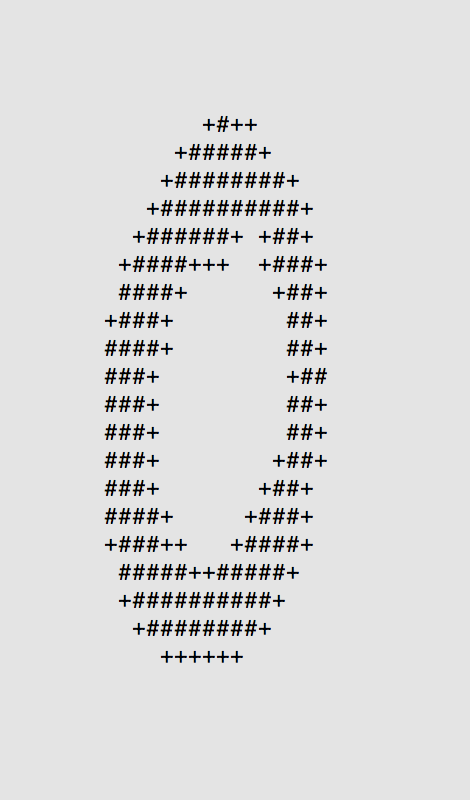
\includegraphics[scale=0.4]{part1/1/high_0.png}

\textbf{Class 0 (Lowest)}\\
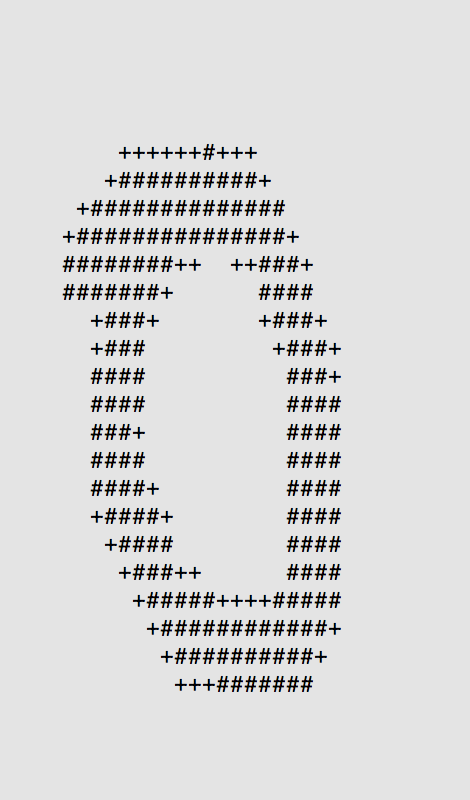
\includegraphics[scale=0.4]{part1/1/low_0.png}
\end{multicols}
\end{center}

\begin{center}
\begin{multicols}{2}
\textbf{Class 1 (Highest)}\\
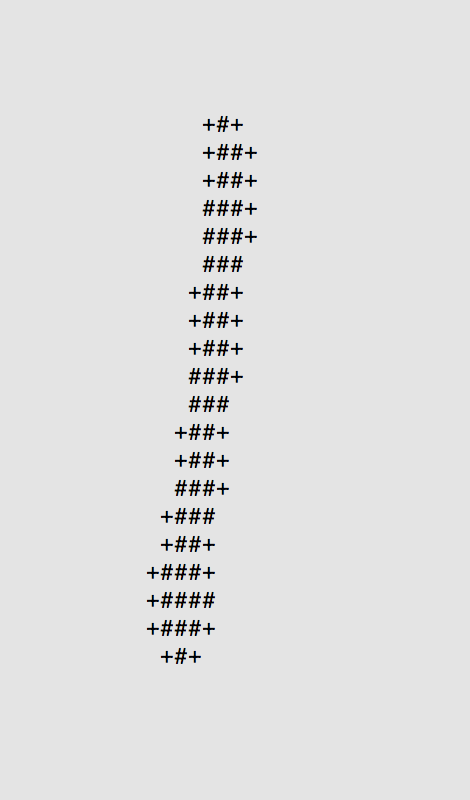
\includegraphics[scale=0.4]{part1/1/high_1.png}

\textbf{Class 1 (Lowest)}\\
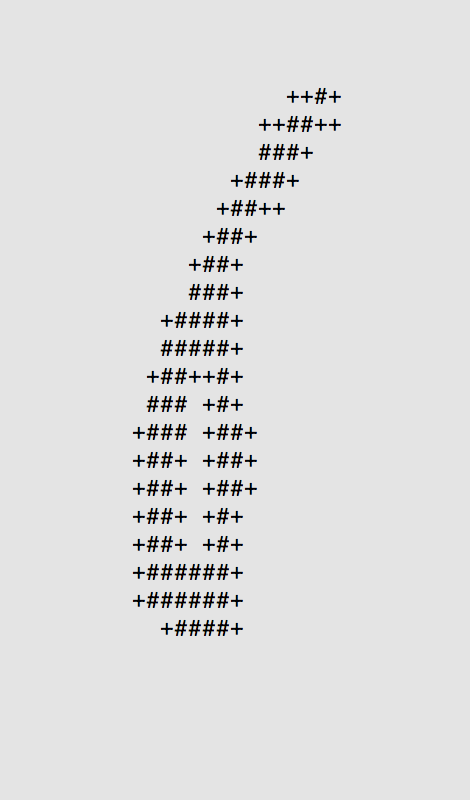
\includegraphics[scale=0.4]{part1/1/low_1.png}
\end{multicols}
\end{center}

\begin{center}
\begin{multicols}{2}
\textbf{Class 2 (Highest)}\\
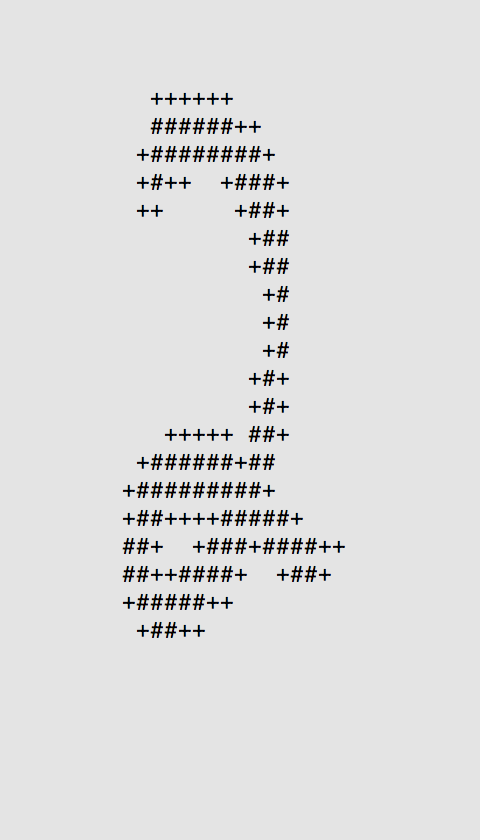
\includegraphics[scale=0.4]{part1/1/high_2.png}

\textbf{Class 2 (Lowest)}\\
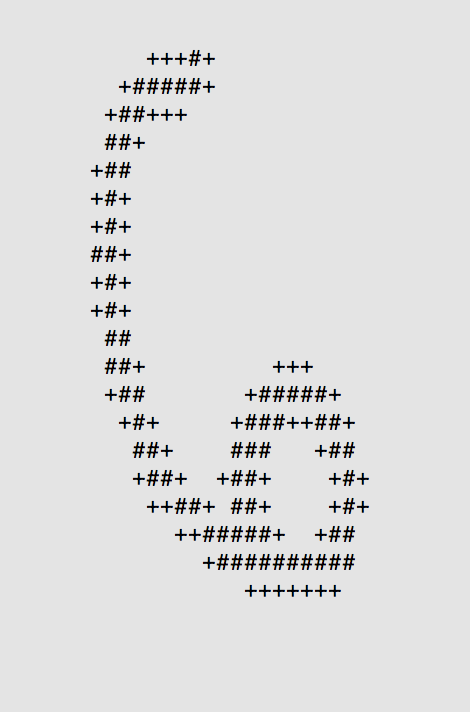
\includegraphics[scale=0.4]{part1/1/low_2.png}
\end{multicols}
\end{center}

\begin{center}
\begin{multicols}{2}
\textbf{Class 3 (Highest)}\\
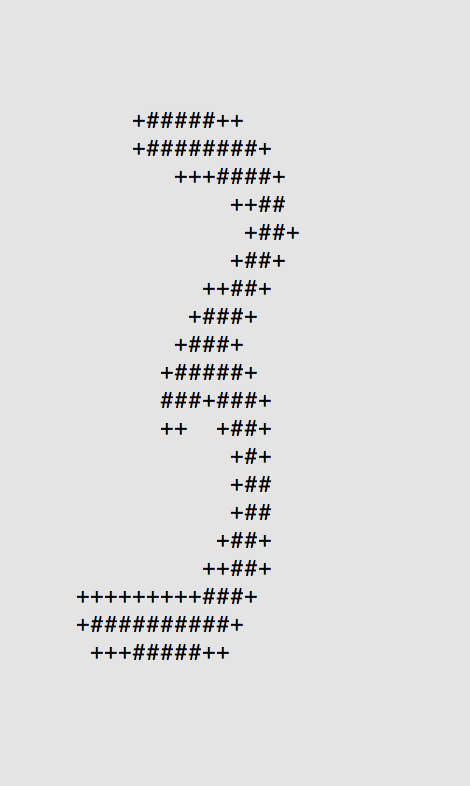
\includegraphics[scale=0.4]{part1/1/high_3.png}

\textbf{Class 3 (Lowest)}\\
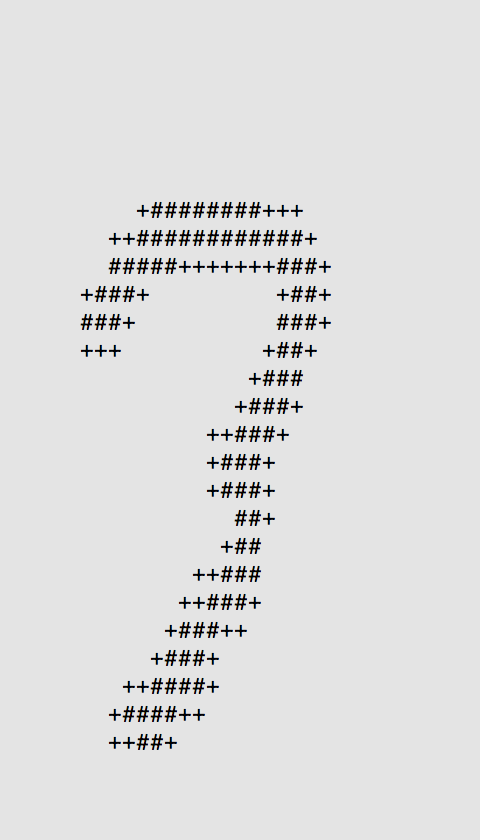
\includegraphics[scale=0.4]{part1/1/low_3.png}
\end{multicols}
\end{center}

\begin{center}
\begin{multicols}{2}
\textbf{Class 4 (Highest)}\\
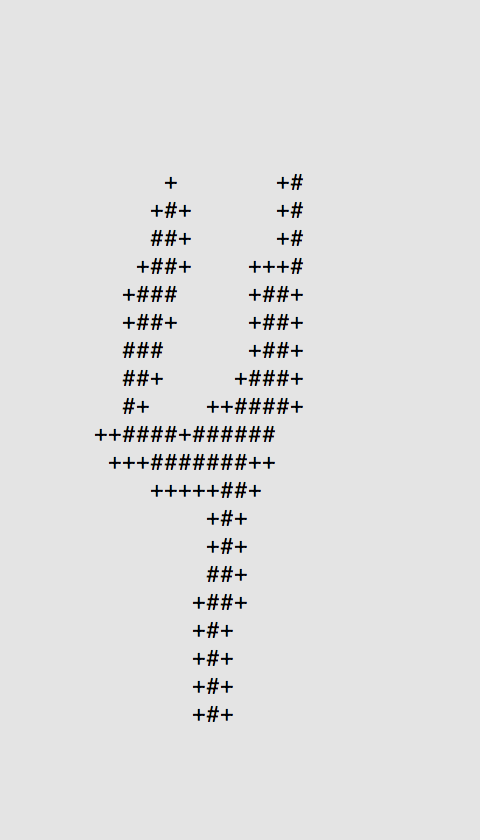
\includegraphics[scale=0.4]{part1/1/high_4.png}

\textbf{Class 4 (Lowest)}\\
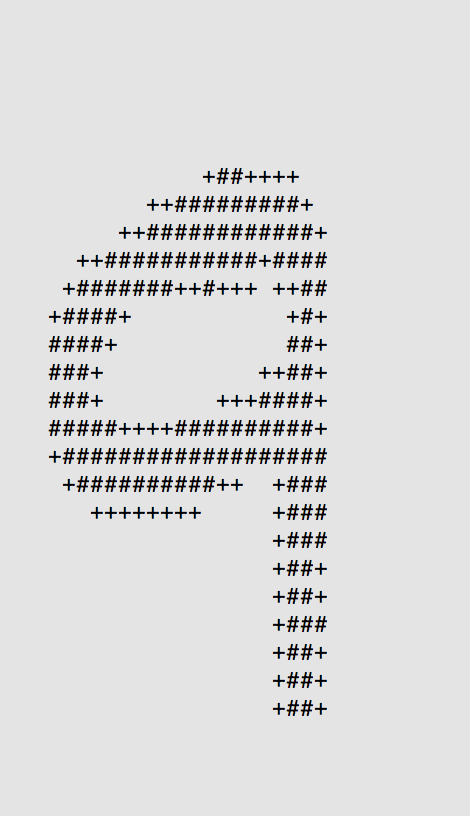
\includegraphics[scale=0.4]{part1/1/low_4.png}
\end{multicols}
\end{center}
\break

\begin{center}
\begin{multicols}{2}
\textbf{Class 5 (Highest)}\\
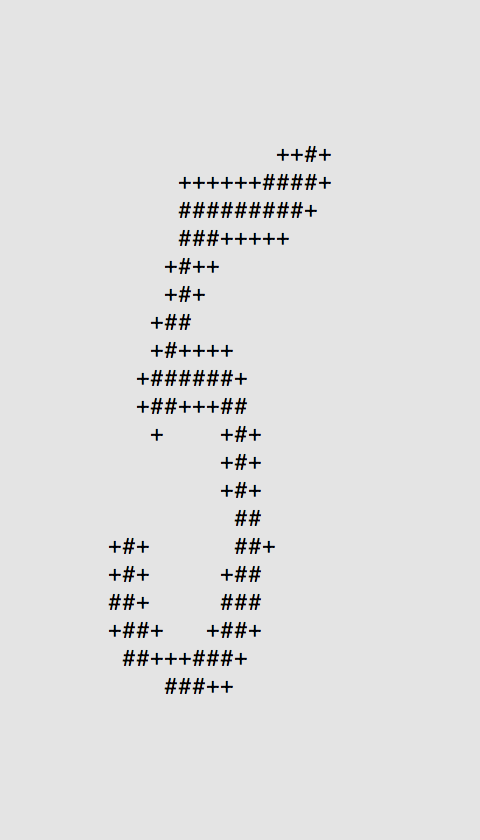
\includegraphics[scale=0.4]{part1/1/high_5.png}

\textbf{Class 5 (Lowest)}\\
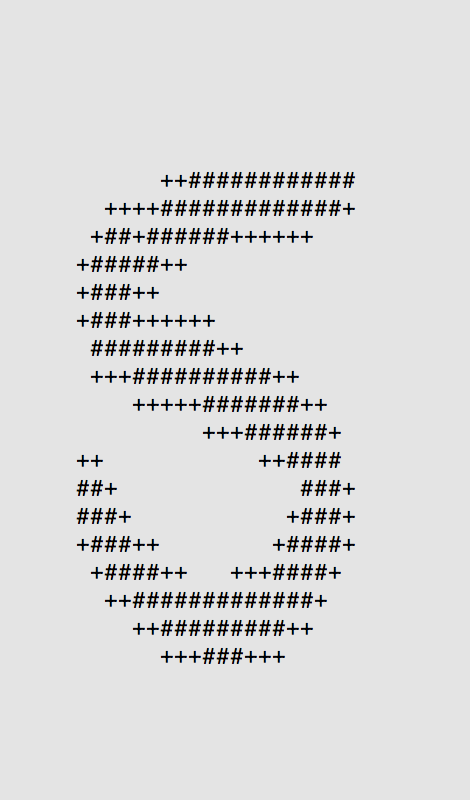
\includegraphics[scale=0.4]{part1/1/low_5.png}
\end{multicols}
\end{center}

\begin{center}
\begin{multicols}{2}
\textbf{Class 6 (Highest)}\\
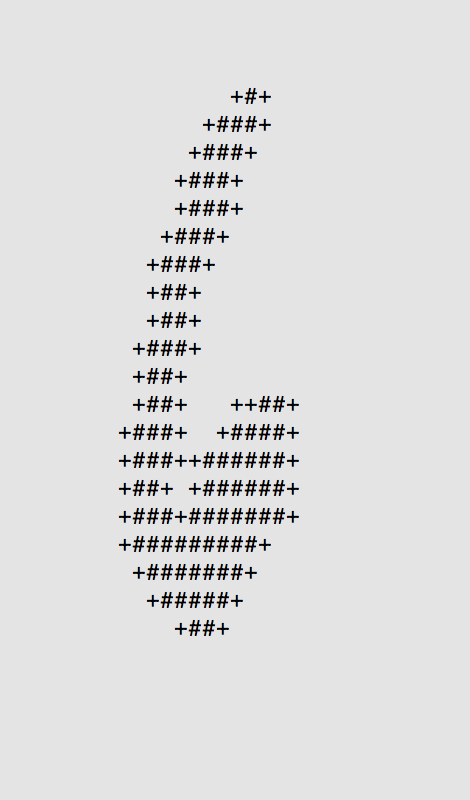
\includegraphics[scale=0.4]{part1/1/high_6.png}

\textbf{Class 6 (Lowest)}\\
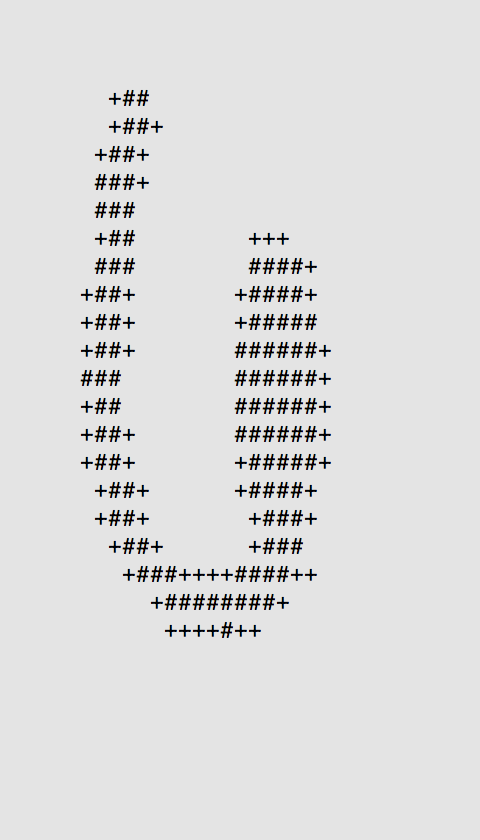
\includegraphics[scale=0.4]{part1/1/low_6.png}
\end{multicols}
\end{center}

\begin{center}
\begin{multicols}{2}
\textbf{Class 7 (Highest)}\\
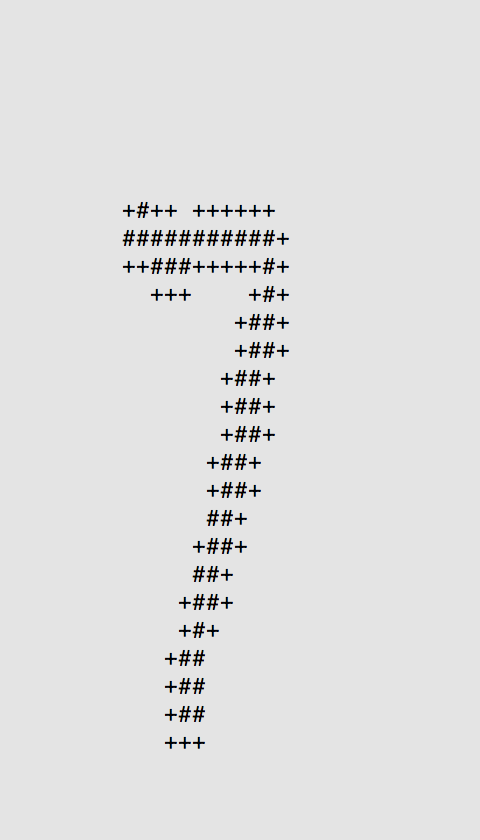
\includegraphics[scale=0.4]{part1/1/high_7.png}

\textbf{Class 7 (Lowest)}\\
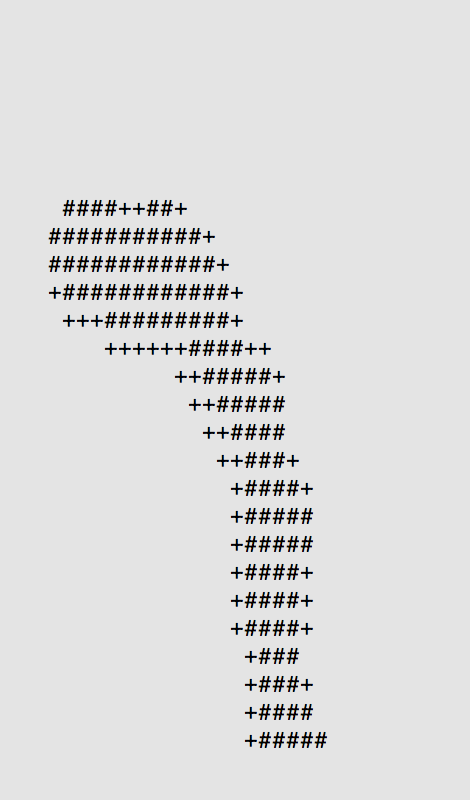
\includegraphics[scale=0.4]{part1/1/low_7.png}
\end{multicols}
\end{center}
\break

\begin{center}
\begin{multicols}{2}
\textbf{Class 8 (Highest)}\\
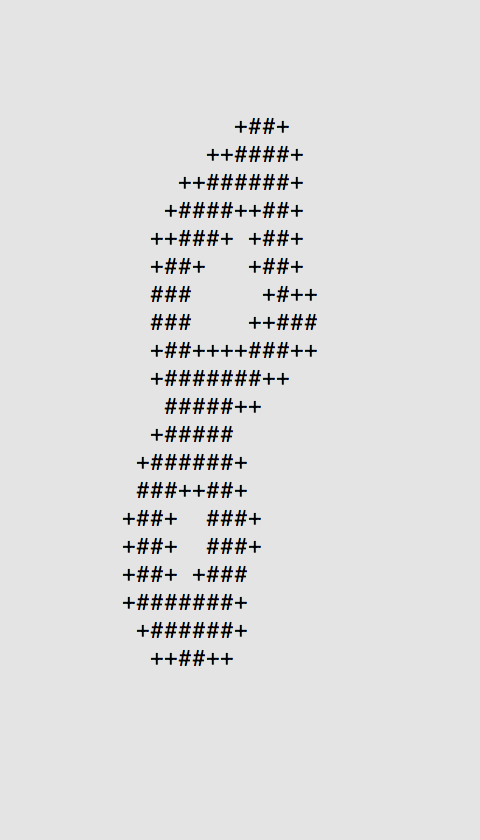
\includegraphics[scale=0.4]{part1/1/high_8.png}

\textbf{Class 8 (Lowest)}\\
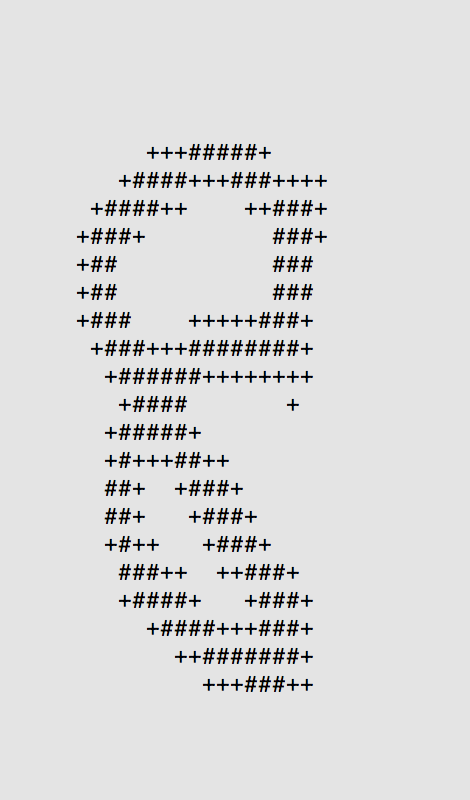
\includegraphics[scale=0.4]{part1/1/low_8.png}
\end{multicols}
\end{center}

\begin{center}
\begin{multicols}{2}
\textbf{Class 9 (Highest)}\\
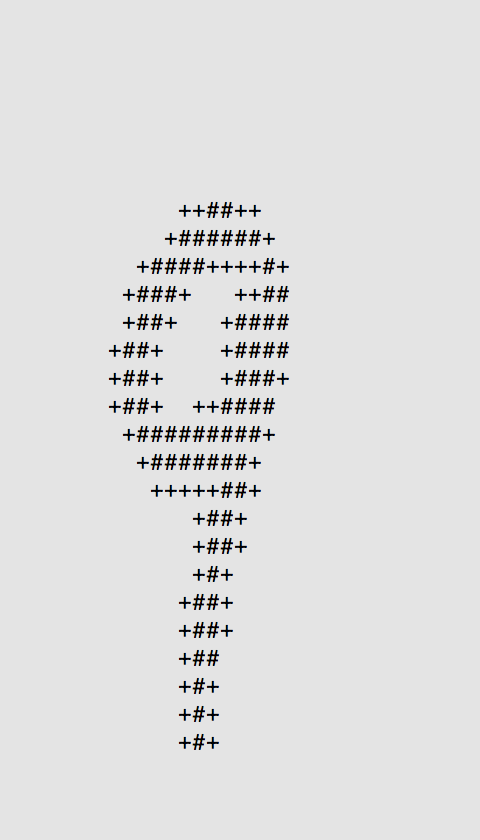
\includegraphics[scale=0.4]{part1/1/high_9.png}

\textbf{Class 9 (Lowest)}\\
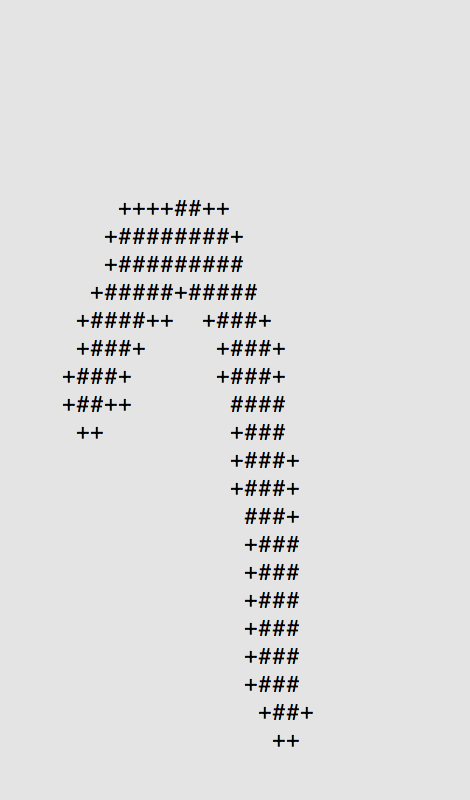
\includegraphics[scale=0.4]{part1/1/low_9.png}
\end{multicols}
\end{center}

\pagebreak
\subsubsection*{Model likelihood and log odd ratios}
Now lets look at the model likelihood for each of the classes with highest confusion rates.\\

\textbf{Class 4 vs Class 9}\\
\begin{center}
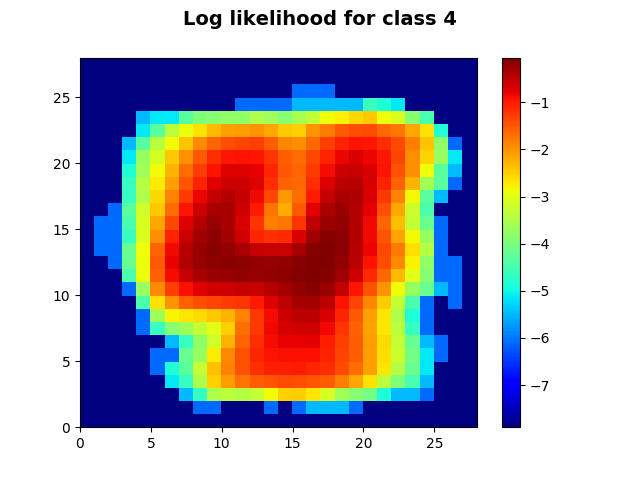
\includegraphics[scale=0.7]{part1/1/log_likelihood_4.png}
\captionof{figure}{Log likelihood of class 4}
\end{center}

\begin{center}
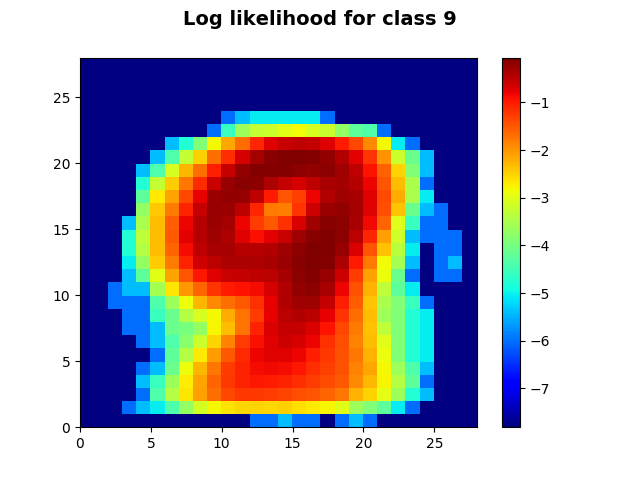
\includegraphics[scale=0.7]{part1/1/log_likelihood_9.png}
\captionof{figure}{Log likelihood of class 9}
\end{center}

\begin{center}
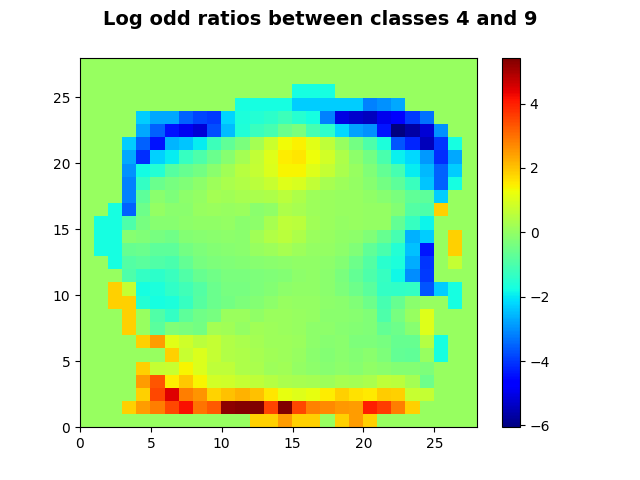
\includegraphics[scale=1]{part1/1/odd_ratio_4_9.png}
\captionof{figure}{Log odd ratio of 4 over 9}
\end{center}

\pagebreak
\textbf{Class 5 vs Class 3}\\
\begin{center}
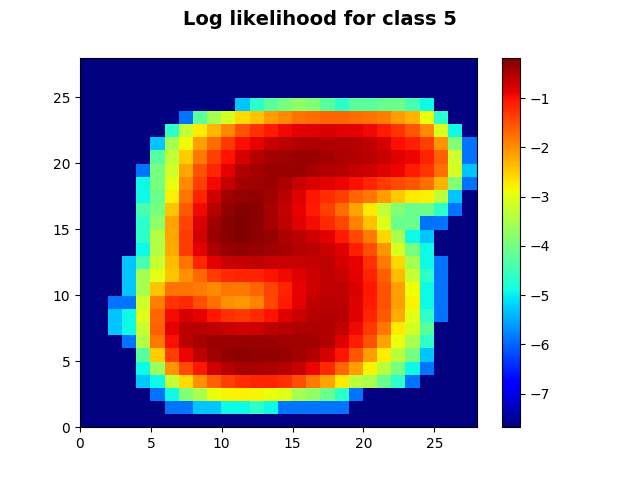
\includegraphics[scale=0.75]{part1/1/log_likelihood_5.png}
\captionof{figure}{Log likelihood of class 5}
\end{center}

\begin{center}
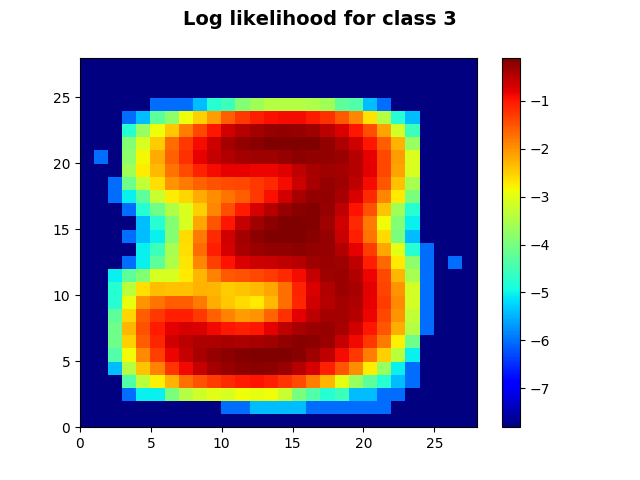
\includegraphics[scale=0.75]{part1/1/log_likelihood_3.png}
\captionof{figure}{Log likelihood of class 3}
\end{center}

\begin{center}
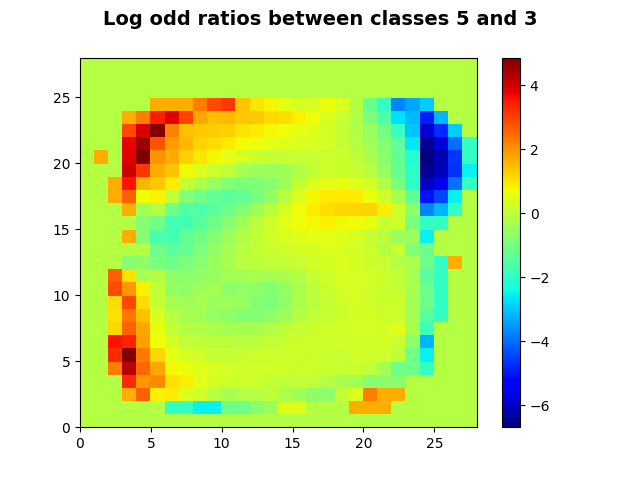
\includegraphics[scale=1]{part1/1/odd_ratio_5_3.png}
\captionof{figure}{Log odd ratio of 5 over 3}
\end{center}

\pagebreak
\textbf{Class 7 vs Class 9}\\
\begin{center}
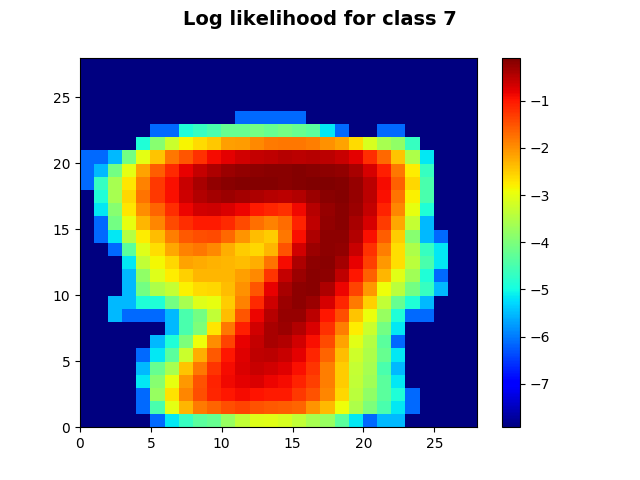
\includegraphics[scale=0.75]{part1/1/log_likelihood_7.png}
\captionof{figure}{Log likelihood of class 7}
\end{center}

\begin{center}
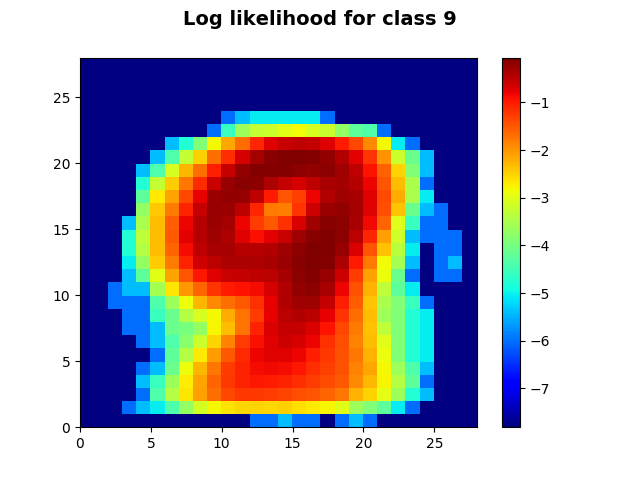
\includegraphics[scale=0.75]{part1/1/log_likelihood_9.png}
\captionof{figure}{Log likelihood of class 9}
\end{center}

\begin{center}
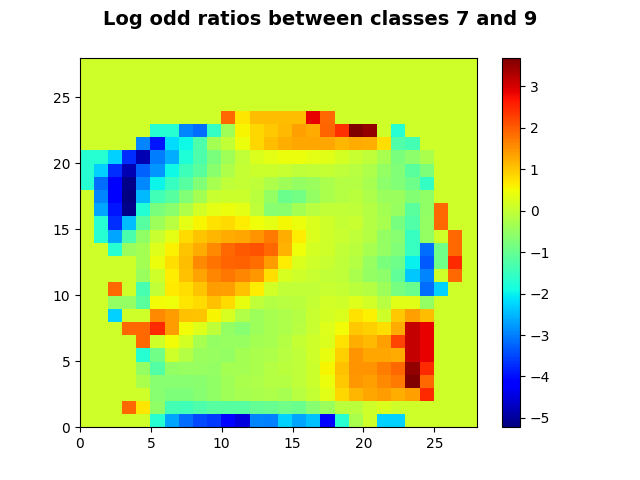
\includegraphics[scale=1]{part1/1/odd_ratio_7_9.png}
\captionof{figure}{Log odd ratio of 7 over 9}
\end{center}

\pagebreak
\textbf{Class 8 vs Class 3}\\
\begin{center}
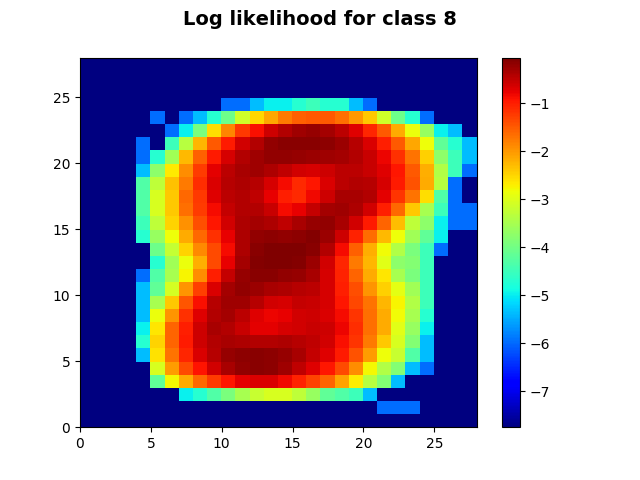
\includegraphics[scale=0.75]{part1/1/log_likelihood_8.png}
\captionof{figure}{Log likelihood of class 8}
\end{center}

\begin{center}
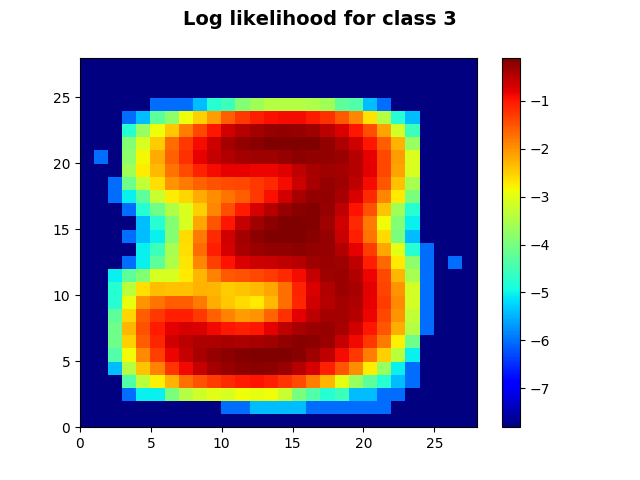
\includegraphics[scale=0.75]{part1/1/log_likelihood_3.png}
\captionof{figure}{Log likelihood of class 3}
\end{center}

\begin{center}
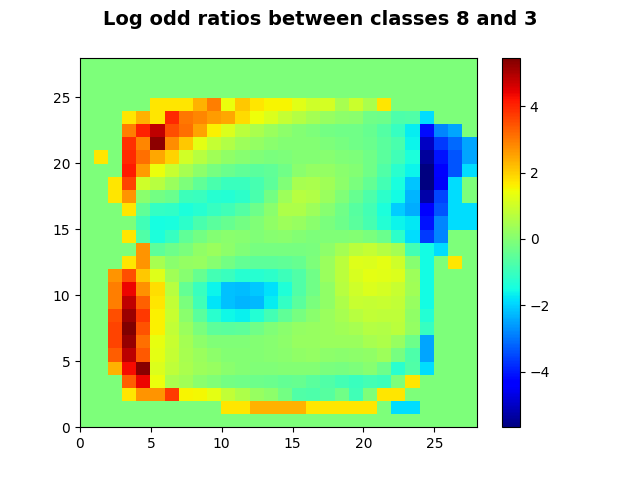
\includegraphics[scale=1]{part1/1/odd_ratio_8_3.png}
\captionof{figure}{Log odd ratio of 8 over 3}
\end{center}

\pagebreak
\subsection*{Part 1.2.}

For this part I set the smoothing constant to 0.001 because, based on part 1.1, it seems like the lower the value the better the accuracy. For the selected group we would have a small matrix, the feature is the result of traversing the matrix from left to right, top to bottom and create a string with the binary values in that order.

\subsubsection*{Disjoint groups of pixels}
I trained my classifier using disjoint groups of pixels of size 2x2, 2x4, 4x2 and 4x4. Here are the results.\\

\begin{center}
\begin{tabular}{cc|r|r|r|r|l}
\cline{3-6}
& & \multicolumn{4}{ c| }{Measure} \\ \cline{3-6}
& & Accuracy & Train time & Eval time & Feature count \\ \cline{1-6}
\multicolumn{1}{ |c  }{\multirow{5}{*}{Size} } &
\multicolumn{1}{ |r| }{1x1} & 77.4\% & 13.08s & 11.21s & 784   \\ \cline{2-6}
\multicolumn{1}{ |c  }{}                        &
\multicolumn{1}{ |r| }{2x2} & 86.7\% & 5.68s & 3.52s & 196    \\ \cline{2-6}
\multicolumn{1}{ |c  }{}                        &
\multicolumn{1}{ |r| }{2x4} & 89.1\% & 3.55s & 1.95s & 98   \\ \cline{2-6}
\multicolumn{1}{ |c  }{}                        &
\multicolumn{1}{ |r| }{4x2} & 89.6\% & 3.9s & 2.04s & 98   \\ \cline{2-6}
\multicolumn{1}{ |c  }{}                        &
\multicolumn{1}{ |r| }{4x4} & 87.3\% & 3.1s & 1.23s & 49   \\ \cline{1-6}
\end{tabular}
\captionof{table}{Summary of performance for different pixel group sizes.}
\end{center}

\subsubsection*{Overlapping groups of pixels}
First I tried multiple group size of overlapping group size and measured the accuracy, training and evaluation time. The results are presented in the following table.

\begin{center}
\begin{tabular}{cc|r|r|r|r|l}
\cline{3-6}
& & \multicolumn{4}{ c| }{Measure} \\ \cline{3-6}
& & Accuracy & Train time & Eval time & Feature count \\ \cline{1-6}
\multicolumn{1}{ |c  }{\multirow{8}{*}{Size} } &
\multicolumn{1}{ |r| }{1x1} & 77.4\% & 13.02s & 11.89s & 784    \\ \cline{2-6}
\multicolumn{1}{ |c  }{}                        &
\multicolumn{1}{ |r| }{2x2} & 89.1\% & 18.98s & 14.14s & 729    \\ \cline{2-6}
\multicolumn{1}{ |c  }{}                        &
\multicolumn{1}{ |r| }{2x4} & 90.2\% & 24.35s & 15.05s & 675   \\ \cline{2-6}
\multicolumn{1}{ |c  }{}                        &
\multicolumn{1}{ |r| }{4x2} & 90.8\% & 26.70s & 15.97s & 675    \\ \cline{2-6}
\multicolumn{1}{ |c  }{}                        &
\multicolumn{1}{ |r| }{4x4} & 91.2\% & 34.61s & 17.09s & 625    \\ \cline{2-6}
\multicolumn{1}{ |c  }{}                        &
\multicolumn{1}{ |r| }{2x3} & 90.4\% & 21.26s & 14.12s & 702    \\ \cline{2-6}
\multicolumn{1}{ |c  }{}                        &
\multicolumn{1}{ |r| }{3x2} & 90.4\% & 23.87s & 15.12s & 702    \\ \cline{2-6}
\multicolumn{1}{ |c  }{}                        &
\multicolumn{1}{ |r| }{3x3} & 91.6\% & 27.01s & 16.01s & 676     \\ \cline{1-6}
\end{tabular}
\captionof{table}{Summary of performance for different pixel group sizes.}
\end{center}

Now lets look at some of the trends on these results.\\
\begin{center}
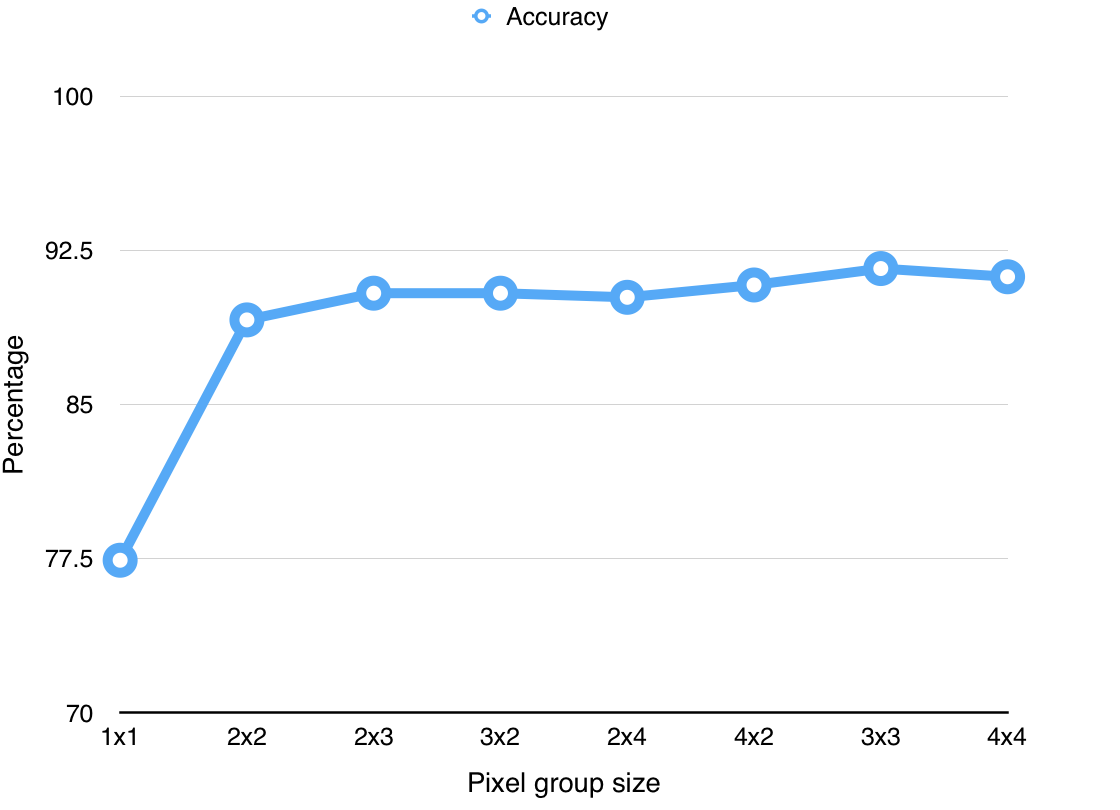
\includegraphics[scale=0.8]{part1/2/overlap_accuracy_2.png}
\captionof{figure}{Line chart for the accuracy of different group sizes.}
\end{center}

The group sizes were sorted increasingly based on the number of pixels in the group. \\
Overall, it seems that the accuracy is positively correlated to the size of the group. Which makes sense but if we were to keep increasing the size we may end up over-fitting our data. For our particular data, 3x3 seems to be a good size.\\

Now, lets see the training time.
\begin{center}
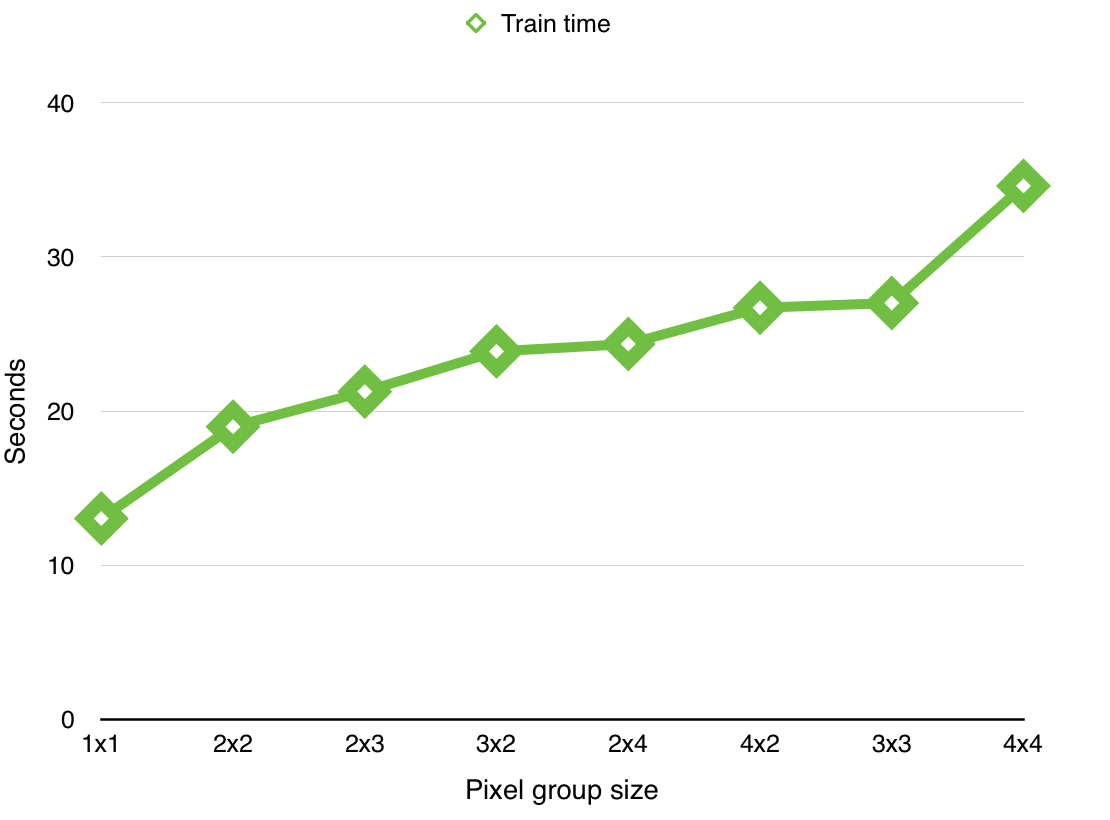
\includegraphics[scale=0.8]{part1/2/overlap_train_2.png}
\captionof{figure}{Line chart for the training time of different group sizes.}
\end{center}

Again, it seems to be a positive correlation between group size and the time it takes the model to train. This makes sense because, as explained in the assignment description, when using a $n$x$m$ group size we would have $2^{nm}$ different values.

Finally, this is how the test time is impacted.
\begin{center}
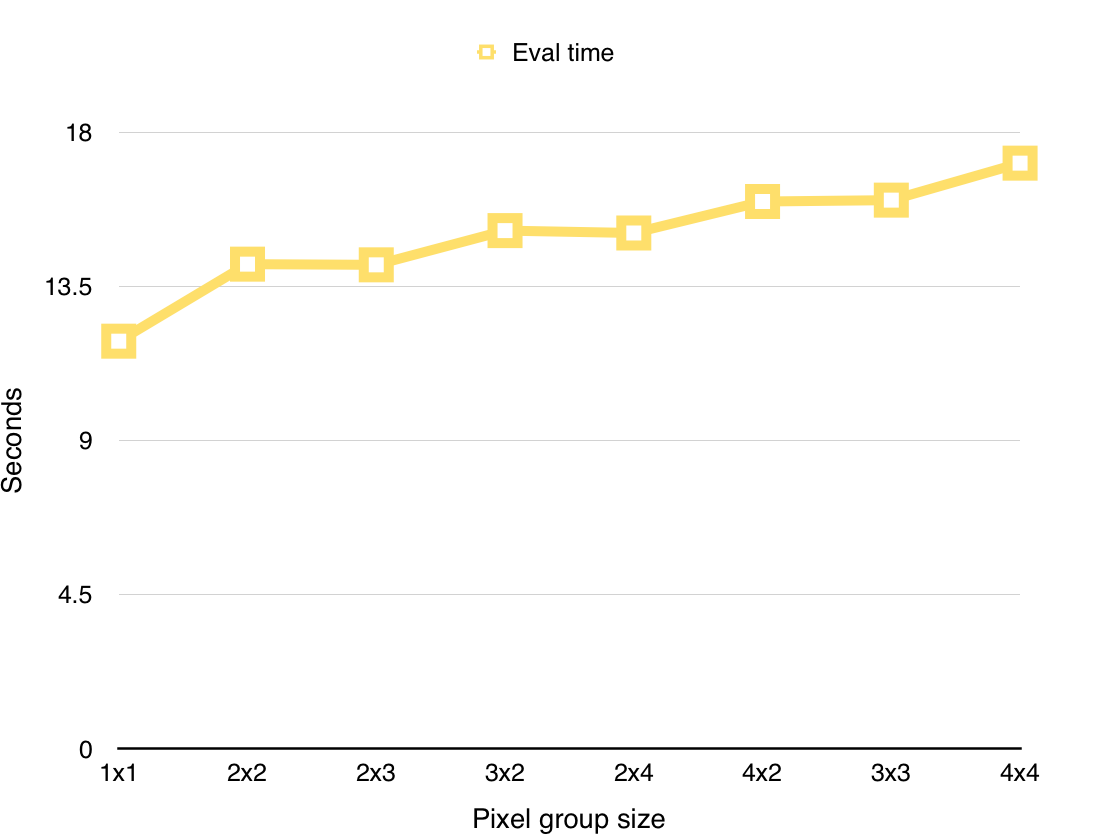
\includegraphics[scale=0.8]{part1/2/overlap_eval_2.png}
\captionof{figure}{Line chart for the evaluation time of different group sizes.}
\end{center}

The evaluation time does increase as the size of the group increased because there are more features to evaluate but note that its growth seems to be slower, probably linear, compared to the previous two measurements.\\

In all cases, going from single pixel to 2x2 represents a very significant improvement.\\

\textbf{Why this works?}\\
Having a bigger group size means that the feature can encode information like the convexity of a portion of the image (the bottom part of digit 8 for example) and the existence of line segments (strokes for digits 4 and 7 for instance). This creates more ways to differentiate between similar digits.\\

\textbf{Note:} more details on each of the trials can be found under the \textit{results} folder. This includes the most and least prototypical digits per class and the confusion matrix.

\subsubsection*{Disjoint vs Overlapping comparison}
Now lets see how performance differs depending on which type of grouping we use.\\

This is a plot of the accuracy for both types:
\begin{center}
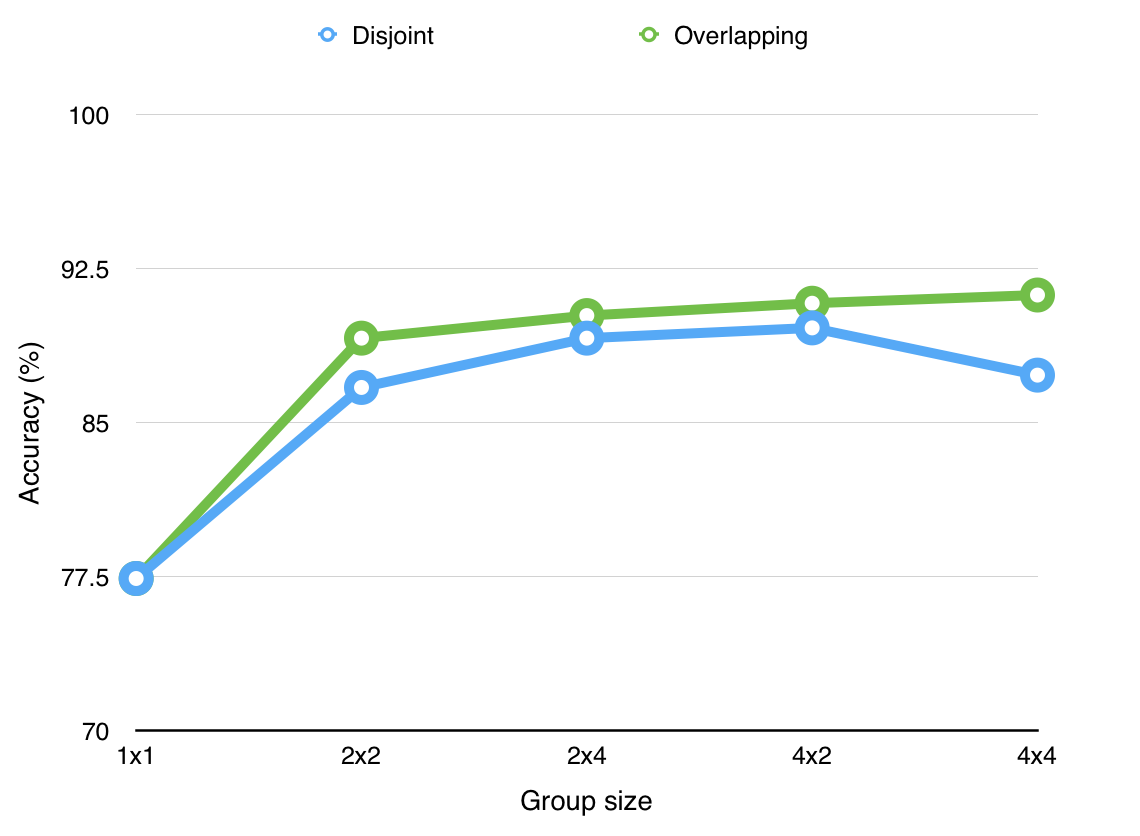
\includegraphics[scale=0.8]{part1/2/comparison_accuracy.png}
\captionof{figure}{Line chart comparing accuracy of overlapping vs disjoint grouping.}
\end{center}

We can see that using overlapping groups outperforms disjoint groups on every size. Not by much though. I think this happens for two reasons: (1) by overlapping we are relaxing the independence condition of Naive Bayes and (2) the number of features is greater.\\

And now lets look at the training time.
\begin{center}
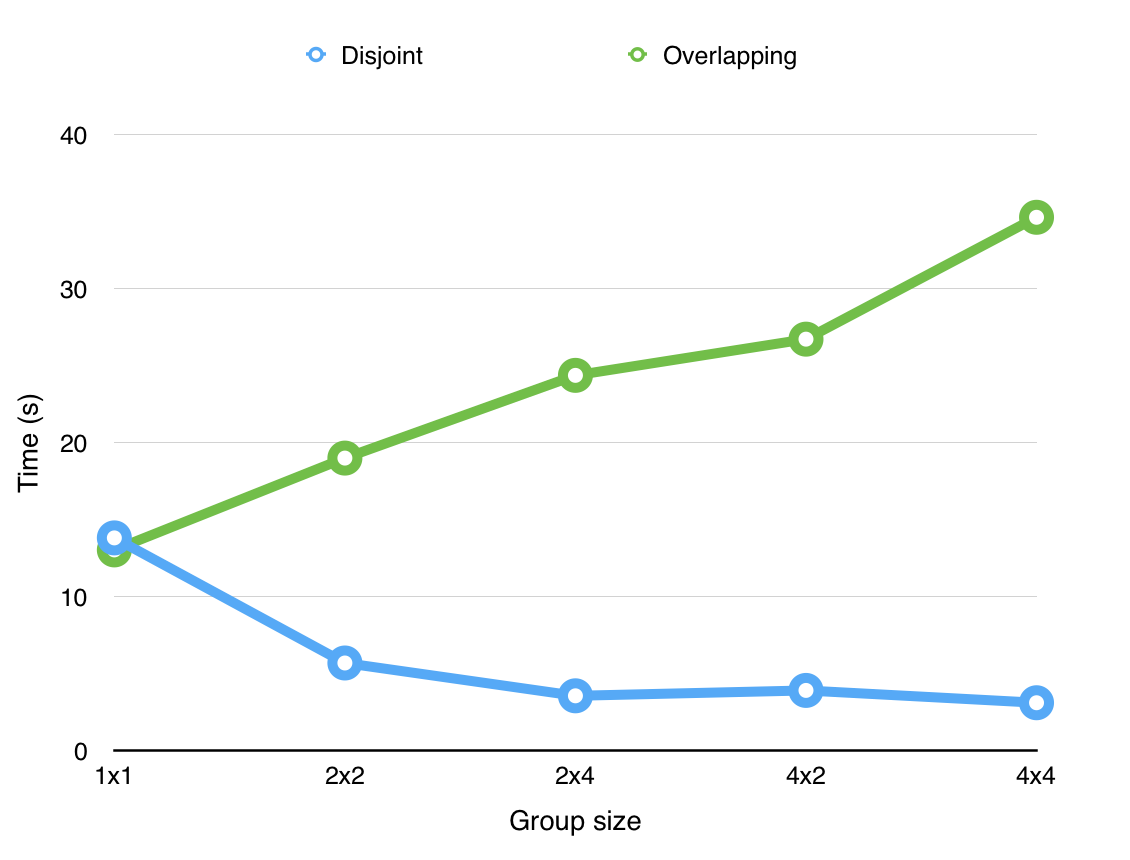
\includegraphics[scale=0.8]{part1/2/comparison_train.png}
\captionof{figure}{Line chart comparing training time of overlapping vs disjoint grouping.}
\end{center}

As expected, the training time for the disjoint groups is way lower than for the overlapping ones. The reason is that the greater the size of the group, the less disjoint groups there will be.\\

At the end of the day, it is always a trade-off between speed and accuracy. If I had to choose one for this dataset I'd chose the disjoint ones because it runs as much as 10 times faster and the accuracy is still within acceptable ranges.\\

\subsubsection*{Time vs feature count}
Finally, lets have a look at how the training time relates to the number of features.

For overlapping groups:\\
\begin{center}
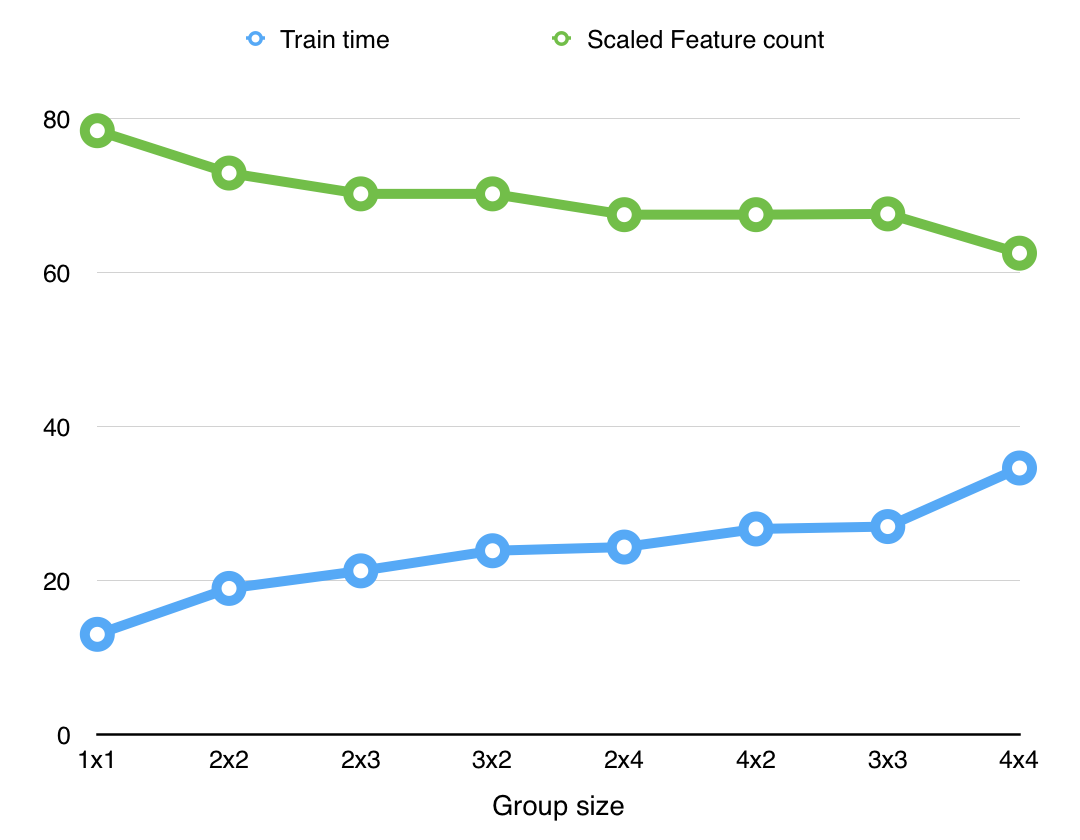
\includegraphics[scale=0.8]{part1/2/overlap_time_feature.png}
\captionof{figure}{Line chart showing the relation between training time and feature count. \\Note: feature count has been scaled by 0.1 so that the chart will be more readable.}
\end{center}

The reasoning for this relation is that even though the number of features is decreasing, it doesn't decrease too fast and, in the meanwhile, the information each feature encodes is greater so it takes longer to create the feature.

For disjoint groups:\\
For overlapping groups:\\
\begin{center}
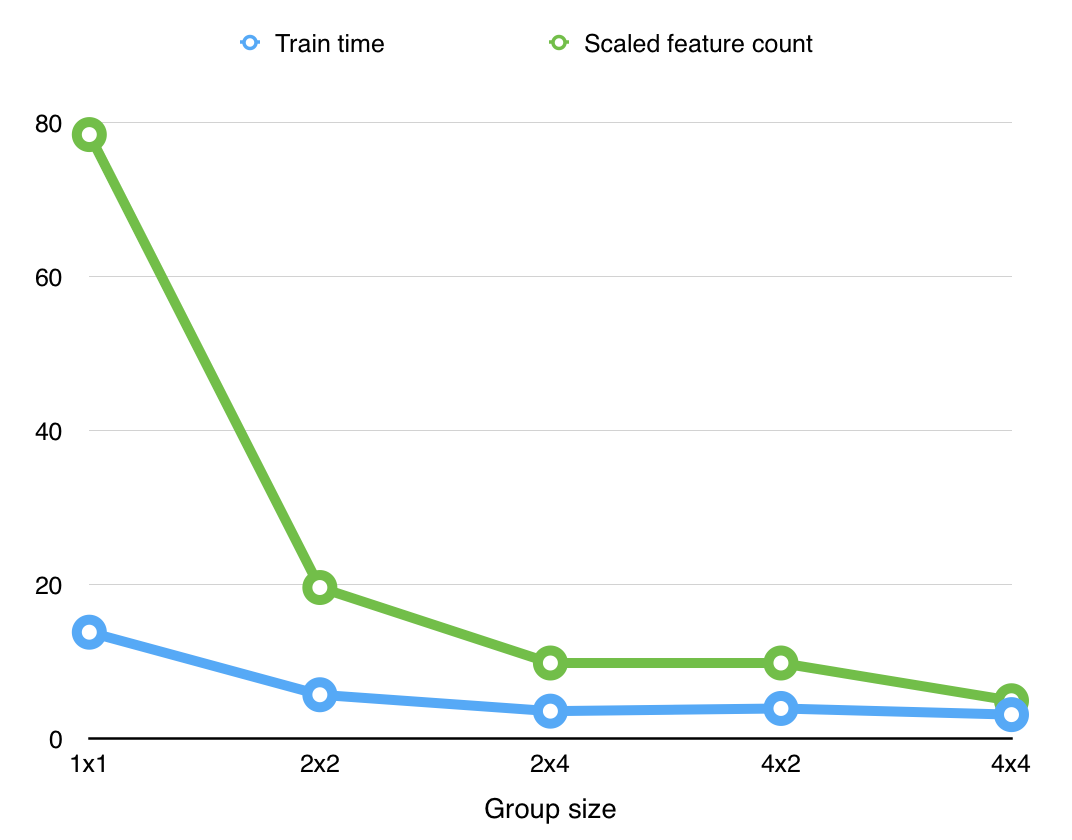
\includegraphics[scale=0.8]{part1/2/disjoint_time_feature.png}
\captionof{figure}{Line chart showing the relation between training time and feature count. \\ Feature count has been scaled by 0.1 so that the chart will be more readable.}
\end{center}

Just like for overlapping groups, the information each feature encodes is greater but in this case the number of features decreases very quickly compared to the overlapping case and therefore the training time decreases.

\subsection*{Extra Credit}
For the first extra credit I implemented the recommended ternary features. \\
For this I created a new class called \textbf{TernaryFeatureExtractor} which uses the three different values found on each example (+, \# and space). It also support pixel grouping. The statistics shown here are the result of using a 3x3 pixel group size and a smoothing constant of 0.001. These values were chosen based on the results obtained from the previous sections.\\

I tried two variations of my \textbf{TernaryFeatureExtractor}:\\
\textbf{Ternary only}: when traversing the pixel group I just take the pixel type and concatenate to create the feature.\\
Using this feature I could never get the accuracy over 89\%, tried the same group sizes from part 1.2 and different smoothing constants but it never went higher.

\textbf{Ternary and binary}: instead of just using the new ternary features I use double amount of features and add back the binary features from part 1.1 and 1.2. Using this finally got the accuracy to 90.2\%. \\

The performance was better than part 1.1 but not better than part 1.2. This is the confusion matrix.\\

\begin{center}

\begin{tabular}{cc|r|r|r|r|r|r|r|r|r|r|l}
\cline{3-12}
& & \multicolumn{10}{ c| }{Predicted class} \\ \cline{3-12}
& & 0 & 1 & 2 & 3 & 4 & 5 & 6 & 7 & 8 & 9  \\ \cline{1-12}
\multicolumn{1}{ |c  }{\multirow{10}{*}{Class} } &
\multicolumn{1}{ |r| }{0} & 96.7 & 0 & 0 & 0 & 0 & 0 & 1.11 & 0 & 2.22 & 0    \\ \cline{2-12}
\multicolumn{1}{ |c  }{}                        &
\multicolumn{1}{ |c| }{1} & 0 & 96.3 & 0.93 & 0 & 0.93 & 0 & 0.93 & 0 & 0.93 & 0    \\ \cline{2-12}
\multicolumn{1}{ |c  }{}                        &
\multicolumn{1}{ |c| }{2} & 0.97 & 0 & 91.26 & 0.97 &  0 & 0 & 1.94 & 0.97 & 3.88 & 0    \\ \cline{2-12}
\multicolumn{1}{ |c  }{}                        &
\multicolumn{1}{ |c| }{3} & 0 & 0 & 1 & 92 &  0 & 3 & 0 & 1 & 1 & 2    \\ \cline{2-12}
\multicolumn{1}{ |c  }{}                        &
\multicolumn{1}{ |c| }{4} & 0 & 0 & 0 & 0 &  94.39 & 0 & 1.87 & 0.93 & 0 & 2.8    \\ \cline{2-12}
\multicolumn{1}{ |c  }{}                        &
\multicolumn{1}{ |c| }{5} & 1.09 & 0 & 1.09 & 4.35 &  0 & 86.96 & 0 & 1.09 & 4.35 & 1.09    \\ \cline{2-12}
\multicolumn{1}{ |c  }{}                        &
\multicolumn{1}{ |c| }{6} & 1.1 & 1.1 & 0 & 0 &  0 & 5.49 & 91.21 & 0 & 1.1 & 0    \\ \cline{2-12}
\multicolumn{1}{ |c  }{}                        &
\multicolumn{1}{ |c| }{7} & 0 & 2.83 & 3.77 & 0 &  0.94 & 0.94 & 0 & 79.25 & 1.89 & 10.38    \\ \cline{2-12}
\multicolumn{1}{ |c  }{}                        &
\multicolumn{1}{ |c| }{8} & 0.97 & 0 & 2.91 & 7.77 &  0.97 & 0.97 & 0 & 0.97 & 85.44 & 0    \\ \cline{2-12}
\multicolumn{1}{ |c  }{}                        &
\multicolumn{1}{ |c| }{9} & 1 & 0 & 0 & 2 &  3 & 1 & 0 & 0 & 4 & 89    \\ \cline{1-12}
\end{tabular}
\captionof{table}{Confusion matrix using smoothing constant 0.001. Values are percentages.}

\end{center}

\section*{Part 2}

\subsection*{Part 2.1}

\subsection*{Part 2.2}

\subsection*{Extra Credit}

\end{document}
